%% ===================================================================
\section{Experiments}\label{sec:experiments}

The propositions assume $\tau^2$ and $M$ known, a Gaussian model and honest participants. Eighteen Monte Carlo simulations, where the truth is known, measure what is lost when each assumption fails; Section~\ref{sec:real} then asks the same of real hospitals. Figure~\ref{fig:sim-forest} places every scenario on one axis and Table~\ref{tab:sims} lists questions and answers; the supplement gives each design in full.

\subsection{Design of the simulation study}\label{sec:sim-design}

Unless stated otherwise the network has 24 hospitals of 16 to 479 patients (log-normal, median 100), $\sigma^2=1$, $C=1$, $\epsilon=1$, $\delta=10^{-5}$, and releases are averaged by 60 gossip rounds on the ring with two-hop links of Figure~\ref{fig:gossip}. Errors are relative to local estimation, so values below 1 mean that hospitals gain. The simulations were built for GHB-lite, whose theory is that of Section~\ref{sec:model}; GHB was added to the logistic comparisons (Simulations 8, 10, 11 and 15) without changing anything else. These worlds favour GHB-lite on purpose: its public feature distribution is exactly that of every hospital, and 24 hospitals of about a hundred patients make its releases informative enough to learn $\tau$. Every baseline spends the same budget under zero-concentrated accounting, and its hyperparameters are tuned on separate replicates with access to the true loss, which no deployment has; GHB and GHB-lite tune nothing. Results are means with $\pm2$ standard errors.

\begin{figure}[t]
\centering
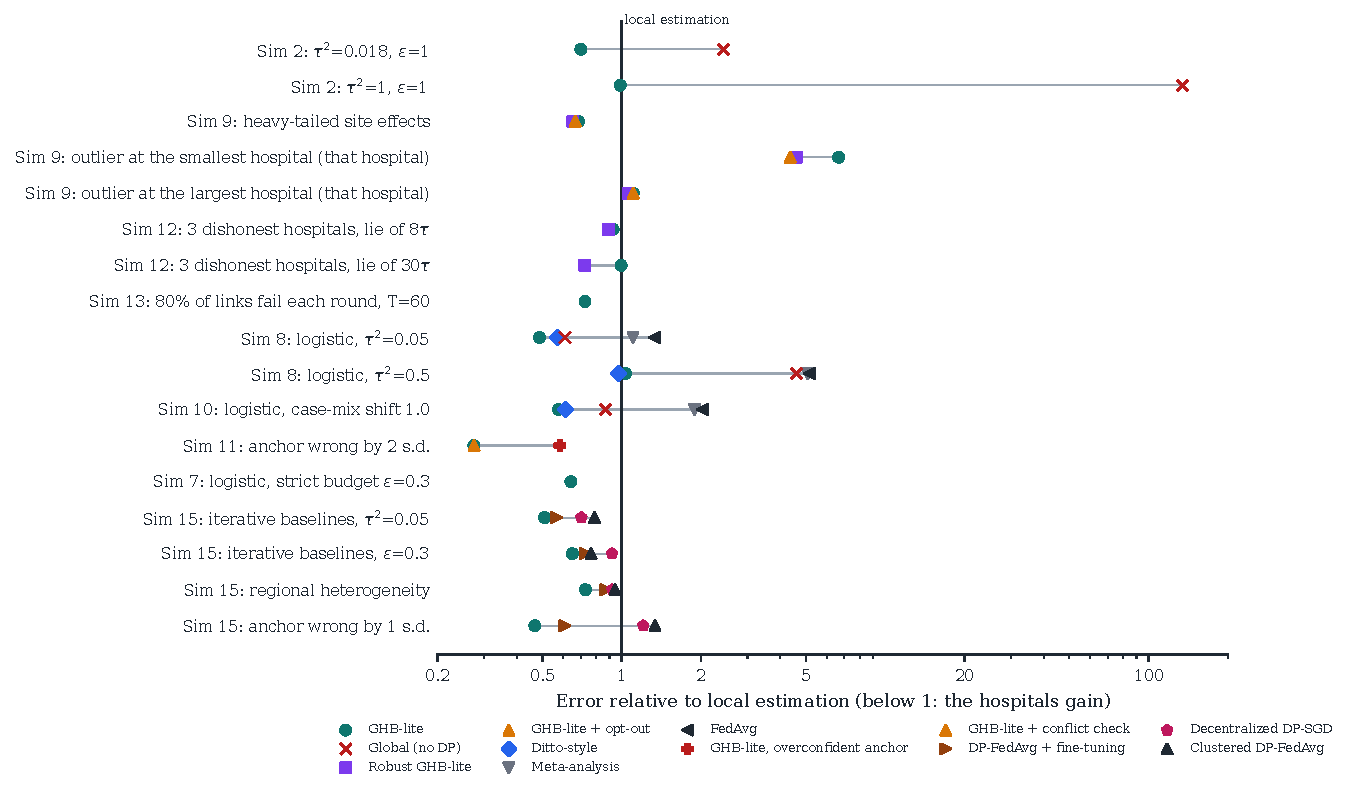
\includegraphics[width=\linewidth]{supplement/figures/sim_forest}
\caption{Summary of Simulations 2 to 15. Each row is a scenario and each marker a method; the horizontal position is the method's error relative to local estimation (mean risk $R_k/v_k$ in the Gaussian simulations, mean excess log-loss divided by that of local estimation in the logistic ones). Left of the vertical line, the hospitals gain. Rows marked ``that hospital'' report the outlying hospital alone.}
\label{fig:sim-forest}
\end{figure}
\begin{table}[t]
\caption{The eighteen simulations, the held-out real networks, and their main results. The simulations run GHB-lite; where GHB was added, its value follows (``GHB''). Relative risk is $R_k/v_k$ and logistic results are mean excess log-loss (nats); below the local value, hospitals gain. $\epsilon=1$ unless stated.}
\label{tab:sims}
\scriptsize
\begin{tabularx}{\linewidth}{@{}>{\raggedright\arraybackslash}p{2.2cm}>{\raggedright\arraybackslash}p{3.3cm}X@{}}
\toprule
Simulation & Question & Result\\
\midrule
1 Closed forms & Do Propositions~\ref{prop:borrowing} and~\ref{prop:privatized} match simulation? & \SimOneWithin{} of \SimOneChecks{} comparisons within two standard errors; largest relative deviation \SimOneMaxRel\\
2 Heterogeneity & Is plug-in GHB-lite ever worse than local estimation? & Worst hospital at most \SimTwoWorstGHB{} for $\tau^2\in[10^{-4},1]$; a global model reaches \SimTwoWorstPool\\
3 Equity, network size & Who gains, and how many hospitals are needed? & Gain in $n^{\eff}$ \SimThreeSmall{} for small, \SimThreeLarge{} for large hospitals; with 3 hospitals relative risk \SimThreeKThreeDL{} against \SimThreeKThreeOracle{} with known $\tau^2$\\
4 Gossip rounds & How many rounds are needed? & Within 2\% of exact averaging after \SimFourRandomTwo{} to \SimFourRingTwo{} rounds, against \SimFourRandomPred{} to \SimFourRingPred{} from the worst-case bound\\
5 Joint release & Does secure aggregation among small hospitals help? & Only if all hospitals are small: $B$ from \SimFiveSmallGOneEpsTenth{} to \SimFiveSmallGEightEpsTenth{} at $\epsilon=0.1$; from \SimFiveMixedGOneEpsTenth{} to \SimFiveMixedGEightEpsTenth{} in a mixed network\\
6 Regional structure & When does the GMRF prior of Equation~\eqref{eq:gmrf} pay off? & Worse when regions barely differ (\SimSixGMRFLow{} against \SimSixGHBLow), far better when they differ (\SimSixGMRFHigh{} against \SimSixGHBHigh)\\
7 Logistic heads & Does it work beyond the Gaussian model? & \SimSevenLocal{} local, \SimSevenGHB{} GHB-lite, \SimSevenGlobal{} pooled without privacy; \SimSevenGHBTenth{} against \SimSevenLocalTenth{} at $\epsilon=0.3$\\
8 Federated baselines & Does it beat existing approaches at the same budget? & At $\tau^2=0.05$: GHB-lite \SimEightMidGHB, GHB \SimEightMidV, Ditto-style \cite{li2021ditto} \SimEightMidDitto, meta-analysis \SimEightMidMeta, FedAvg \cite{mcmahan2017communication} \SimEightMidFedavg; at $\tau^2=0.5$ GHB-lite \SimEightHighGHB{} against local \SimEightHighLocal\\
9 Atypical hospitals & What happens to a hospital unlike the others? & Heavy tails: \SimNineTGHB, robust prior \SimNineTRobust; an outlier at the smallest hospital loses (\SimNineSmallGHB, at best \SimNineSmallOpt), at the largest barely (\SimNineLargeGHB)\\
10 Case-mix shift & Does it survive hospitals with different patients? & Shift of one s.d.: GHB-lite \SimEightShiftGHB, GHB \SimEightShiftV, Ditto-style \cite{li2021ditto} \SimEightShiftDitto, pooled \SimEightShiftPooled, local \SimEightShiftLocal\\
11 Wrong anchor & What if the published model is wrong? & Honest uncertainty or a conflict check: at most \SimElevenHonestMax{} at any error; an overconfident anchor \SimElevenOverTwo{} at 2 s.d.; GHB at most \SimElevenVMax\\
12 Dishonest hospitals & What if hospitals lie? & Plain GHB-lite never above \SimTwelveWorstGHB; robust screening keeps \SimTwelveRobustLarge{} against large lies, at a cost of \SimTwelveRobustNone{} against \SimTwelveGHBNone{} when nobody lies\\
13 Link failures & What if links fail during gossip? & With 80\% of links failing each round, \SimThirteenEighty{} after 60 rounds against \SimThirteenExact{} with exact averaging\\
14 Repeated releases & What do refits on the same patients cost? & After \SimFourteenR{} refits, $B=\SimFourteenBasic$ with basic composition and \SimFourteenZcdp{} with zero-concentrated accounting (one release: \SimFourteenOne)\\
15 Iterative federated learning & Does it beat multi-round training with the same budget and tuned hyperparameters? & At $\tau^2=0.05$: GHB-lite \SimFifteenMidGHB, GHB \SimFifteenMidV, DP-FedAvg \cite{mcmahan2018learning} with fine-tuning \SimFifteenMidFT, decentralized DP-SGD \cite{lian2017can} \SimFifteenMidDec, clustered \SimFifteenMidClus; at $\epsilon=0.3$ GHB-lite \SimFifteenStrictGHB{} against \SimFifteenStrictFT; worst hospital at most \SimFifteenGHBWorstMax{} for GHB-lite except at $\tau^2=0.5$, \SimFifteenFTWorstMin{} to \SimFifteenFTWorstMax{} for fine-tuning\\
16 Ablation & What does each component contribute? & Error relative to GHB-lite without it: ridge release up to \SimSixteenRidgeMax; $X^\top y$ release \SimSixteenXtyShift{} under case-mix shift; plug-in $\tau^2$ up to \SimSixteenTauMeanMax{} (posterior mean) and \SimSixteenTauDLMax{} (DerSimonian-Laird \cite{dersimonian1986meta}); no conflict check \SimSixteenNoCheckAnchor{} with a wrong anchor; equal weights up to \SimSixteenEqualMax; gossip and accounting free\\
17 Sensitivity & How much do settings and conditions matter? & Settings: quantiles, public sample, threshold and rounds ($\ge 20$) flat; prior scale of $\tau$ \SimSeventeenScaleMin{} to \SimSeventeenScaleMax; misstated anchor up to \SimSeventeenAnchorSdMax. Conditions: error \SimSeventeenRelMin{} to \SimSeventeenRelMax{} of local, worst hospital at most \SimSeventeenWorstMax\\
16B, 17B GHB & Which of GHB's components and settings matter, and across which conditions? & Intercept borrowed \SimSixteenBIntMin{} to \SimSixteenBIntMax{} of GHB's error (this world shares base rates); no non-borrowing components down to \SimSixteenBSafetyMin; most settings within \SimSixteenBSmallMax; across conditions \SimSeventeenBRelMin{} to \SimSeventeenBRelMax{} of local, worst hospital at most \SimSeventeenBWorstMax\\
18 Group fairness & What does borrowing do to a protected group? & Minority excess log-loss ($\times10^{-3}$) with a shared disparity: GHB-lite \SimEighteenSharedGHBMin, local \SimEighteenSharedLocalMin, FAIR-FATE \cite{salazar2023fairfate} \SimEighteenSharedFFEQOMin; disparities that vary: GHB-lite \SimEighteenVariesGHBMin, global \SimEighteenVariesGlobalMin; equalized odds of GHB-lite within 0.02 of the true models, FAIR-FATE closer to parity\\
Real data & Does it hold on real hospitals, against the literature tuned as a consortium could? & Five held-out TCGA networks: GHB \SimTCOneGHB{} and \SimTCTenGHB{} relative to local at $\epsilon=1$ and 10; best literature method \SimTCOneFT{} and \SimTCTenDitto{} (Section~\ref{sec:real})\\
\bottomrule
\end{tabularx}
\end{table}

\subsection{Does the theory survive estimation?}\label{sec:sim-theory}

A real network must estimate $\tau^2$ and $M$ from privatized releases, so the first question is how much of the predicted gain survives, and for whom. Simulation 1 confirms the closed forms. Across four orders of magnitude of heterogeneity (Simulation 2, Figure~\ref{fig:sim-het}), plug-in GHB-lite stays at or below local estimation for every hospital, while a global model becomes up to \SimTwoMeanPool{} times worse on average and \SimTwoWorstPool{} times worse for its worst hospital; the price of estimating $\tau^2$ appears only when heterogeneity is tiny (\SimTwoMinGHB{} against \SimTwoMinOracle{} with the true value). Gossip is free once mixed: 11 to 35 rounds suffice on the topologies of Figure~\ref{fig:gossip} (Simulation 4), and mixing survives 80\% of links failing each round (\SimThirteenEighty{} against \SimThirteenExact, Simulation 13).

\begin{figure}[t]
\centering
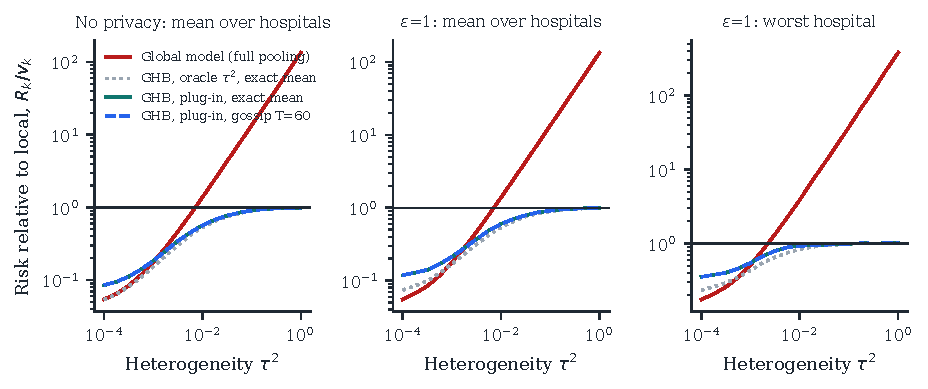
\includegraphics[width=\linewidth]{supplement/figures/s2_heterogeneity}
\caption{Simulation 2: risk relative to local estimation against heterogeneity, for 24 hospitals of 16 to 479 patients. Plug-in GHB-lite estimates $\tau^2$ and $M$ from privatized releases averaged by gossip; the oracle uses the true $\tau^2$; the global model is the sample-size weighted mean of all site estimates, computed without privacy.}
\label{fig:sim-het}
\end{figure}

Who gains is what (R4) asks. Every hospital gains about $B\approx\SimThreeB$ virtual patients (Simulation 3, Figure~\ref{fig:sim-equity}), so hospitals of 60 patients or fewer multiply their effective sample size by \SimThreeSmall{} and those of 300 or more by \SimThreeLarge; a global model helps small hospitals less (\SimThreePoolSmall) and cuts large ones to \SimThreePoolLarge{} of their own. With three hospitals, $\tau^2$ is too poorly estimated and most of the gain is lost; a half-Cauchy prior helps from four upward.

\begin{figure}[t]
\centering
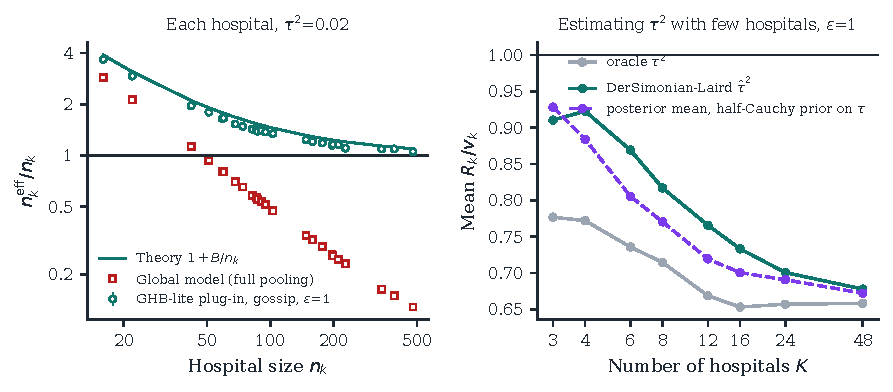
\includegraphics[width=\linewidth]{supplement/figures/s3_equity}
\caption{Simulation 3. Left: effective sample size relative to own size for each hospital at $\tau^2=0.02$, $\epsilon=1$; the line is $1+B/n_k$ from Equation~\eqref{eq:borrowed}. Right: mean relative risk against the number of hospitals for three ways of obtaining $\tau^2$.}
\label{fig:sim-equity}
\end{figure}

\subsection{Against federated and meta-analytic baselines}\label{sec:sim-baselines}

Gaining over local estimation matters only if the method also beats what a network could adopt instead. From here on the heads are logistic regressions on four features, every baseline consumes the same budget, and its hyperparameters are tuned on the true loss.

\paragraph{One-shot baselines} Simulations 8 and 10 compare methods that use the same releases (Figure~\ref{fig:sim-baselines}, Table~\ref{tab:sim8}). At $\tau^2=0.05$ GHB-lite reaches \SimEightMidGHB, below a Ditto-style \cite{li2021ditto} model tuned on separate replicates (\SimEightMidDitto) and below a global model trained on pooled data without privacy (\SimEightMidPooled); federated averaging \cite{mcmahan2017communication} and meta-analysis, which give every hospital one model, are worse than local (\SimEightMidFedavg{} and \SimEightMidMeta{} against \SimEightMidLocal). Under case-mix shift GHB-lite keeps its lead (\SimEightShiftGHB{} against \SimEightShiftDitto). From $\tau^2=0.2$ the tuned Ditto-style model is slightly better, and at $\tau^2=0.5$ it is the only method that gains. GHB is less accurate than GHB-lite here (\SimEightMidV{} at $\tau^2=0.05$), for two reasons that are this world's: it cannot learn $\tau$ from per-hospital releases, and these hospitals differ in base rate no more than in slopes, so not borrowing the intercept costs rather than protects.

\begin{figure}[t]
\centering
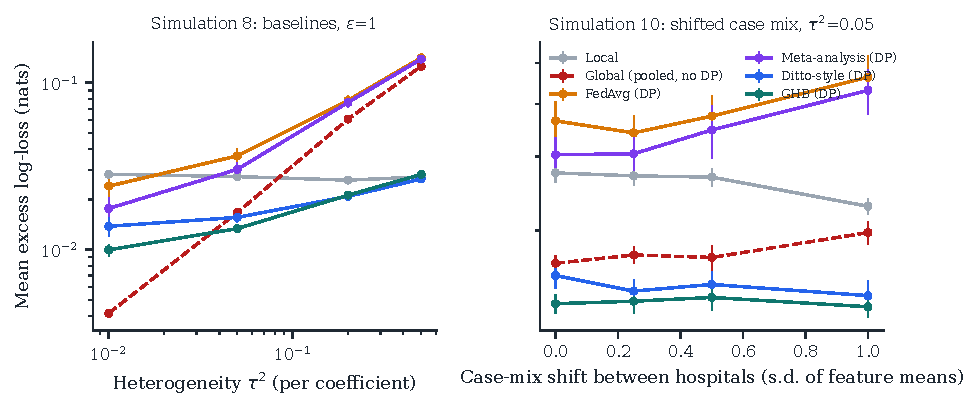
\includegraphics[width=\linewidth]{supplement/figures/sim8_baselines}
\caption{Simulations 8 and 10, logistic-regression heads. Mean excess log-loss over the true model of GHB-lite, of private baselines that use the same releases (one-shot federated averaging \cite{mcmahan2017communication}, random-effects meta-analysis, Ditto-style \cite{li2021ditto} personalization tuned on separate replicates) and of a global model trained on the pooled data without privacy. Left: against coefficient heterogeneity. Right: against case-mix shift between hospitals at $\tau^2=0.05$. Bars: $\pm 2$ standard errors.}
\label{fig:sim-baselines}
\end{figure}
\begin{table}[t]
\caption{Simulations 8 and 10: exact values behind Figure~\ref{fig:sim-baselines}. Values are mean excess log-loss in $10^{-3}$ nats, with two Monte Carlo standard errors in grey; the lowest private method in each row is bold. All private methods use the same releases at $\epsilon=1$; the pooled model uses no privacy. GHB (joint releases) appears in the table but not in the figure.}
\label{tab:sim8}
\scriptsize
\setlength{\tabcolsep}{4pt}
\begin{tabular}{@{}lrrrrrrr@{}}
\toprule
Setting & Local & GHB & GHB-lite & \makecell[r]{Ditto-style\\\cite{li2021ditto}} & \makecell[r]{Meta-analysis\\\cite{dersimonian1986meta}} & \makecell[r]{FedAvg\\\cite{mcmahan2017communication}} & Pooled, no DP\\
\midrule
\csname @@input\endcsname../Collectively_Big_Locally_Small/supplement/results/tables/t_sim8.tex 
\bottomrule
\end{tabular}
\end{table}

\paragraph{Iterative federated learning} Simulation 15 faces multi-round training: DP-FedAvg \cite{mcmahan2017communication,mcmahan2018learning} with and without fine-tuning, decentralized DP-SGD \cite{lian2017can} on the same graph, and clustered training in the style of IFCA \cite{ghosh2020efficient}, all tuned on \SimFifteenTune{} replicates with the true loss (Figure~\ref{fig:sim-literature}, Tables~\ref{tab:sim15} and~\ref{tab:sim15worst}); four of the ten settings were held out while GHB-lite was designed. GHB-lite is the most accurate method in six settings, three of them held out, for instance at $\tau^2=0.05$ (\SimFifteenMidGHB{} against \SimFifteenMidFT{} for DP-FedAvg with fine-tuning) and at $\epsilon=0.3$ (\SimFifteenStrictGHB{} against \SimFifteenStrictFT); the tuned Ditto-style model is slightly better at $\tau^2=0.2$, without privacy and with a wrong anchor, and at $\tau^2=0.5$ nothing beats local estimation. Its gain at a strict budget comes from borrowing, not the anchor: a tuned local control started from the anchor reaches \SimFifteenStrictAnchorGD{} and becomes worse than local when the anchor is wrong (\SimFifteenAnchorAnchorGD). GHB, with joint releases, does less well in this world, whose hospitals share their base rates: significantly better than local estimation in \SimStSimLocBetter{} of \SimStSimLocN{} settings, but worse than the tuned Ditto-style model in \SimStSimDittoWorse{} and than DP-FedAvg with fine-tuning in \SimStSimFTWorse{} (supplement).

The methods differ most in who pays. GHB-lite's worst hospital stays within a factor \SimFifteenGHBWorstMax{} of its local error in every private setting except $\tau^2=0.5$; fine-tuning leaves some hospital \SimFifteenFTWorstMin{} to \SimFifteenFTWorstMax{} times worse off, usually a large one whose data the federated model overrides (the eight largest go from \SimFifteenStrictLocalLarge{} alone to \SimFifteenStrictFTLarge{} at $\epsilon=0.3$, against \SimFifteenStrictGHBLarge{} with GHB-lite). What remains is the cost of not knowing $\tau^2$: with the true value GHB-lite would reach \SimFifteenStrictOracle{} at $\epsilon=0.3$. GHB, for the reasons above, beats every iterative baseline in \SimFifteenVBeatsIter{} of the ten settings and trails GHB-lite in all ten (\SimFifteenMidV{} at $\tau^2=0.05$), with its worst hospital within a factor \SimFifteenVWorstMax{} of its local error. In worlds where GHB-lite's inversion is exact, per-hospital releases are worth their noise; Section~\ref{sec:real} shows that on real hospitals they were not.

\begin{figure}[t]
\centering
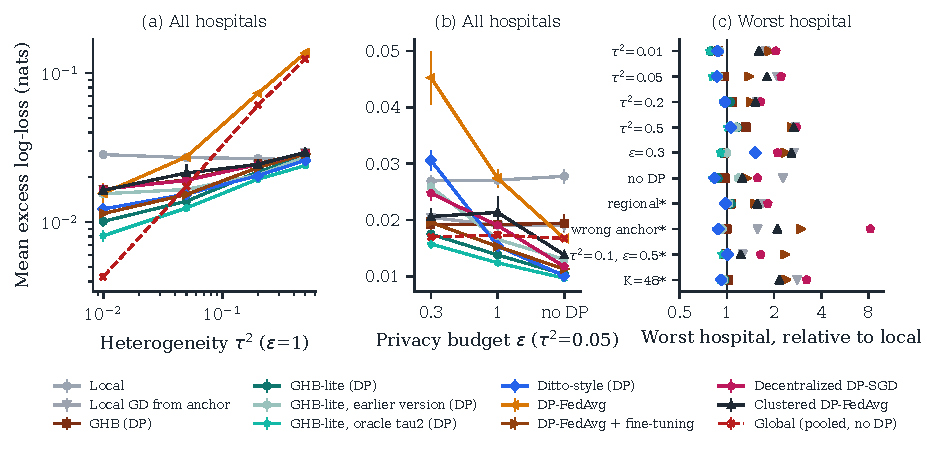
\includegraphics[width=\linewidth]{supplement/figures/sim15_literature}
\caption{Simulation 15: GHB-lite against iterative federated learning at the same privacy budget (logistic heads, 24 hospitals, mean excess log-loss over \SimFifteenReps{} replicates, $\pm2$ standard errors). Baseline hyperparameters are tuned with access to the true loss; GHB-lite is not tuned. (a) Against heterogeneity at $\epsilon=1$. (b) Against the privacy budget at $\tau^2=0.05$. (c) The worst hospital's error relative to its own local estimate in each setting; right of 1, some hospital is worse off than alone; settings marked $\ast$ were held out while GHB-lite was designed. ``GHB-lite, earlier version'' is an earlier formulation that released ridge fits, shown for reference; ``GHB-lite, oracle $\tau^2$'' uses the true heterogeneity and is a reference, not a method.}
\label{fig:sim-literature}
\end{figure}
\begin{table}[t]
\caption{Simulation 15: exact values behind Figure~\ref{fig:sim-literature}. Values are mean excess log-loss in $10^{-3}$ nats, with two Monte Carlo standard errors in grey; the lowest private method in each row is bold. Settings marked $\ast$ were held out while GHB-lite was designed. FT: fine-tuning \cite{mcmahan2018learning}. The figure's marker labelled GHB is GHB-lite; GHB (joint releases) appears in the table.}
\label{tab:sim15}
\scriptsize
\setlength{\tabcolsep}{2.2pt}
\resizebox{\linewidth}{!}{\begin{tabular}{@{}lrrrrrrrrrr@{}}
\toprule
Setting & Local & \makecell[r]{Anchor\\GD} & GHB & GHB-lite & \makecell[r]{Ditto-\\style\\\cite{li2021ditto}} & \makecell[r]{DP-FedAvg\\+ FT\\\cite{mcmahan2018learning}} & \makecell[r]{Decentr.\\DP-SGD\\\cite{lian2017can}} & \makecell[r]{Clustered\\DP-FedAvg\\\cite{ghosh2020efficient}} & \makecell[r]{GHB-lite,\\true $\tau^2$} & \makecell[r]{Pooled,\\no DP}\\
\midrule
\csname @@input\endcsname../Collectively_Big_Locally_Small/supplement/results/tables/t_sim15_mean.tex 
\bottomrule
\end{tabular}}
\end{table}
\begin{table}[t]
\caption{Simulation 15: who pays. Left: the largest ratio of any hospital's mean excess log-loss to its own local value (above 1, some hospital is worse off than alone; lowest in bold). Middle: the percentage of hospitals that gain over local estimation. Right: the mean excess log-loss of the eight largest hospitals ($10^{-3}$ nats).}
\label{tab:sim15worst}
\scriptsize
\setlength{\tabcolsep}{2.4pt}
\resizebox{\linewidth}{!}{\begin{tabular}{@{}lrrrrrrrrrrrrrr@{}}
\toprule
 & \multicolumn{8}{c}{Worst hospital, relative to local} & \multicolumn{3}{c}{Hospitals that gain (\%)} & \multicolumn{3}{c}{Eight largest}\\
\cmidrule(lr){2-9}\cmidrule(lr){10-12}\cmidrule(l){13-15}
Setting & Local & \makecell[r]{Anchor\\GD} & GHB & GHB-lite & \makecell[r]{Ditto\\\cite{li2021ditto}} & \makecell[r]{FedAvg\\+ FT\\\cite{mcmahan2018learning}} & \makecell[r]{Decentr.\\\cite{lian2017can}} & \makecell[r]{Clust.\\\cite{ghosh2020efficient}} & GHB-lite & \makecell[r]{Ditto\\\cite{li2021ditto}} & \makecell[r]{FedAvg\\+ FT\\\cite{mcmahan2018learning}} & Local & GHB-lite & \makecell[r]{FedAvg\\+ FT\\\cite{mcmahan2018learning}}\\
\midrule
\csname @@input\endcsname../Collectively_Big_Locally_Small/supplement/results/tables/t_sim15_worst.tex 
\bottomrule
\end{tabular}}
\end{table}

\paragraph{Privacy is the binding constraint} GHB-lite cuts the excess log-loss of local estimation by \SimSevenReduction{} at $\epsilon=1$ and keeps most of that at $\epsilon=0.3$ (\SimSevenGHBTenth{} against \SimSevenLocalTenth, Simulation 7), whereas releasing ridge fits instead of scores kept almost none (\SimFifteenStrictOld): what a hospital releases matters as much as how much privacy it spends. Joint release among groups of small hospitals helps only when every hospital is small (Simulation 5), and refits are affordable only under zero-concentrated accounting: after \SimFourteenR{} refits a hospital keeps $B=\SimFourteenZcdp$ virtual patients, against \SimFourteenBasic{} under basic composition (Simulation 14).

\subsection{What breaks it}\label{sec:sim-attacks}

Next, failures on purpose. \emph{Atypical hospitals} (Simulation 9) are the failure Proposition~\ref{prop:borrowing} predicts. Heavy-tailed effects keep the mean risk low (\SimNineTGHB; \SimNineTRobust{} with a Student-$t$ prior), and an outlying large hospital barely loses (\SimNineLargeGHB), but an outlying small one loses badly (\SimNineSmallGHB{} times its local risk, at best \SimNineSmallOpt{} with any safeguard): a small hospital cannot tell from its own data that it is atypical, and only external structure (Simulation 6, Equation~\eqref{eq:gmrf}) can. \emph{A wrong anchor} (Simulation 11) is harmless when its uncertainty is stated honestly or it is dropped on conflict (at most \SimElevenHonestMax), but an overconfident anchor two standard deviations off raises the error to \SimElevenOverTwo; GHB stays at or below \SimElevenVMax{} at every error. The conflict check is therefore part of both protocols. \emph{Dishonest hospitals} (Simulation 12) never pushed honest ones below local performance: a large lie inflates $\hat{\tau}^2$ and switches borrowing off (worst \SimTwelveWorstGHB), and screening releases keeps the gain against large lies (\SimTwelveRobustLarge) at a small cost when nobody lies.

\subsection{Which components and settings matter}\label{sec:sim-components}

Simulation 16 removes one component of GHB-lite at a time, on the same data and noise (Figure~\ref{fig:sim-ablation}, Table~\ref{tab:sim16}). Every component earns its place somewhere and costs little elsewhere. Releasing a ridge fit instead of the score is worse in seven of eight settings, by up to \SimSixteenRidgeMax; releasing $X^\top y$ is \SimSixteenXtyShift{} times worse under case-mix shift, which the score at the anchor absorbs; inverse-variance weighting is worth up to \SimSixteenEqualMax, the anchor up to \SimSixteenNoAnchorMax, and the conflict check \SimSixteenNoCheckAnchor{} when the anchor is wrong. The rule for $\tau$ is the most delicate: plug-in rules win slightly when hospitals are alike and lose by up to \SimSixteenTauMeanMax{} (posterior mean) or \SimSixteenTauDLMax{} (DerSimonian-Laird \cite{dersimonian1986meta}) elsewhere, while integrating $\tau$ out with each hospital's evidence is within 4\% of the best rule everywhere. Gossip and zero-concentrated accounting cost nothing for a single release.

\begin{figure}[t]
\centering
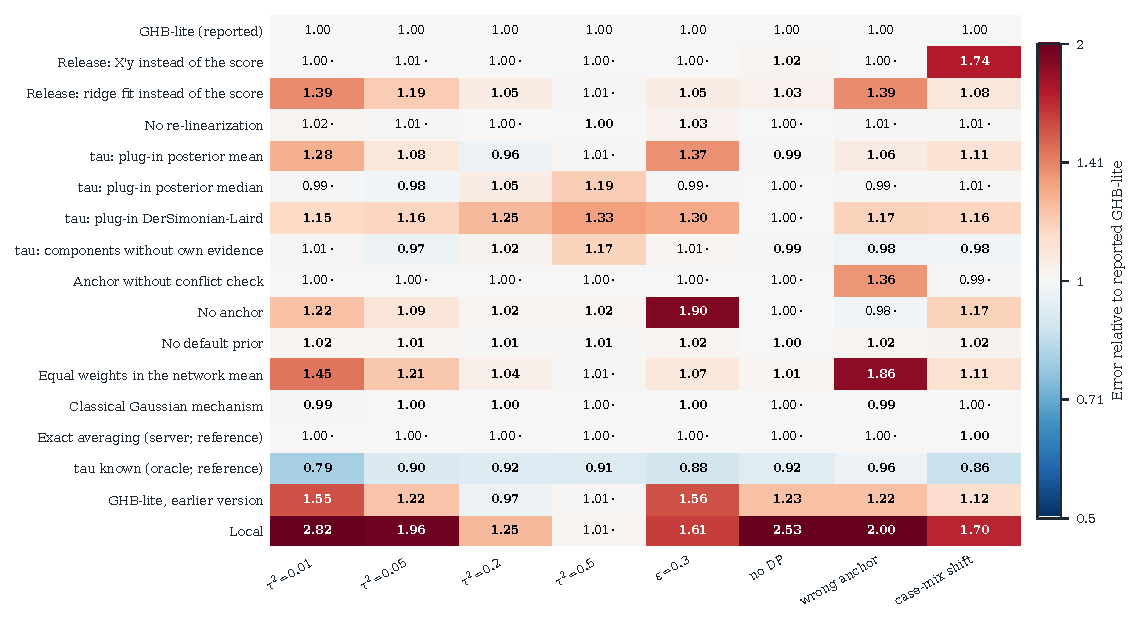
\includegraphics[width=\linewidth]{supplement/figures/sim16_ablation}
\caption{Simulation 16: ablation of GHB-lite (logistic heads, 24 hospitals, \SimSixteenReps{} replicates per setting). Each cell is the mean excess log-loss of a variant divided by that of GHB-lite as reported, computed on the same data and noise; above 1 (red), removing or replacing the component hurts. Bold: paired difference larger than two standard errors; a trailing dot marks differences within Monte Carlo error. The last three rows are references.}
\label{fig:sim-ablation}
\end{figure}
\begin{table}[t]
\caption{Simulation 16: exact values behind Figure~\ref{fig:sim-ablation}. First row: mean excess log-loss of GHB-lite as reported ($10^{-3}$ nats). Other rows: the mean excess log-loss of each variant divided by that of GHB-lite on the same data and noise (\SimSixteenReps{} replicates per setting); bold where the paired difference exceeds two standard errors. The last rows are references.}
\label{tab:sim16}
\scriptsize
\setlength{\tabcolsep}{3pt}
\begin{tabular}{@{}lrrrrrrrr@{}}
\toprule
Variant & $\tau^2=0.01$ & $\tau^2=0.05$ & $\tau^2=0.2$ & $\tau^2=0.5$ & $\epsilon=0.3$ & no DP & \makecell[r]{wrong\\anchor} & shift\\
\midrule
\csname @@input\endcsname../Collectively_Big_Locally_Small/supplement/results/tables/t_sim16.tex 
\bottomrule
\end{tabular}
\end{table}

Simulation 17 varies GHB-lite's own settings and the network around it (Figures~\ref{fig:sim-settings} and~\ref{fig:sim-conditions}, Tables~\ref{tab:sim17a} and~\ref{tab:sim17b}). Most settings hardly matter: the number of quantiles from three, the public sample from 2,000 draws, the conflict threshold from 2.5, gossip from 20 rounds. Two do: the half-Cauchy scale trades nearly identical against heterogeneous hospitals (\SimSeventeenScaleMin{} to \SimSeventeenScaleMax), with the default 0.5 within 11\% of the best everywhere, and an understated anchor uncertainty costs up to \SimSeventeenAnchorSdMax. Across 6 to 96 hospitals, median sizes of 25 to 400, budgets from $\epsilon=0.1$ to none, and every topology, the error stays between \SimSeventeenRelMin{} and \SimSeventeenRelMax{} of local and the worst hospital within a factor \SimSeventeenWorstMax; the gain grows with the number of hospitals and the budget, and is largest for hospitals of about 100 patients.

\begin{figure}[t]
\centering
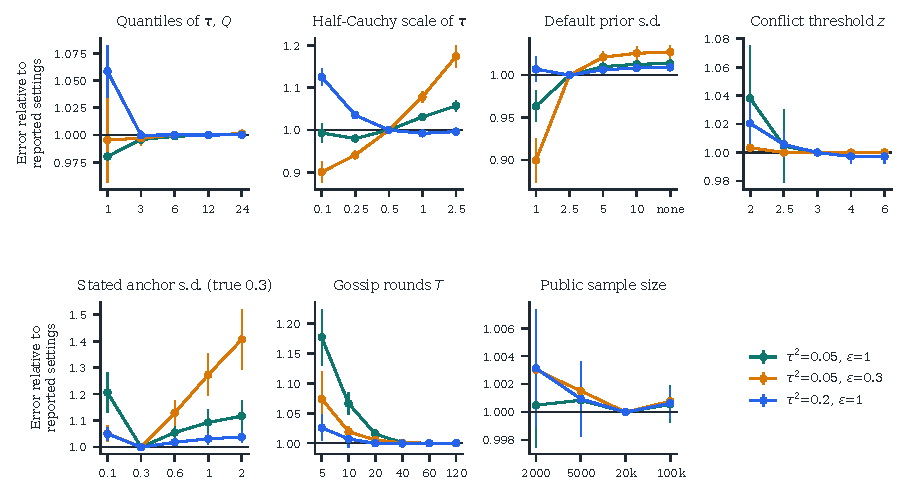
\includegraphics[width=\linewidth]{supplement/figures/sim17_settings}
\caption{Simulation 17, part A: sensitivity of GHB-lite to its own settings (logistic heads, \SimSeventeenReps{} paired replicates per point). Each point is the mean excess log-loss with the setting changed, divided by that with the reported settings ($Q=12$, scale 0.5, default prior s.d.\ 2.5, $z=3$, stated anchor s.d.\ 0.3, $T=60$, 20,000 public draws). Bars: $\pm2$ standard errors of the paired ratio.}
\label{fig:sim-settings}
\end{figure}
\begin{table}[t]
\caption{Simulation 17, part A: exact values behind Figure~\ref{fig:sim-settings}. Mean excess log-loss with one setting changed, divided by that with the reported settings (italic), on the same data and releases; two standard errors of the paired ratio in grey (\SimSeventeenReps{} replicates).}
\label{tab:sim17a}
\scriptsize
\begin{tabular}{@{}llrrr@{}}
\toprule
Setting & Value & $\tau^2=0.05$, $\epsilon=1$ & $\tau^2=0.05$, $\epsilon=0.3$ & $\tau^2=0.2$, $\epsilon=1$\\
\midrule
\csname @@input\endcsname../Collectively_Big_Locally_Small/supplement/results/tables/t_sim17_settings.tex 
\bottomrule
\end{tabular}
\end{table}
\begin{figure}[t]
\centering
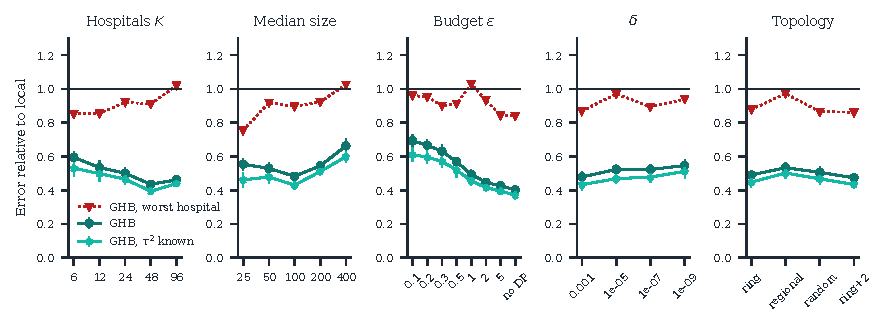
\includegraphics[width=\linewidth]{supplement/figures/sim17_conditions}
\caption{Simulation 17, part B: GHB-lite across network conditions ($\tau^2=0.05$, $\epsilon=1$, 24 hospitals of median size 100 on the ring with two-hop links unless varied; \SimSeventeenReps{} replicates per point). Mean excess log-loss relative to local estimation for GHB-lite and for GHB-lite with $\tau^2$ known ($\pm2$ standard errors), and the largest ratio of any hospital's error to its own local error (dotted).}
\label{fig:sim-conditions}
\end{figure}
\begin{table}[t]
\caption{Simulation 17, part B: exact values behind Figure~\ref{fig:sim-conditions}. Mean excess log-loss of GHB-lite relative to local estimation (two standard errors in grey), the same for GHB-lite with $\tau^2$ known, the largest ratio of any hospital's error to its own local error, and the absolute mean excess log-loss of GHB-lite and of local estimation ($10^{-3}$ nats). $\tau^2=0.05$, $\epsilon=1$, $\delta=10^{-5}$, 24 hospitals of median size 100 on the ring with two-hop links unless varied.}
\label{tab:sim17b}
\scriptsize
\begin{tabular}{@{}llrrrrr@{}}
\toprule
Condition & Value & GHB-lite / local & \makecell[r]{GHB-lite, $\tau^2$ known\\/ local} & Worst hospital & GHB-lite & Local\\
\midrule
\csname @@input\endcsname../Collectively_Big_Locally_Small/supplement/results/tables/t_sim17_conditions.tex 
\bottomrule
\end{tabular}
\end{table}

\paragraph{The same analysis for GHB} Simulation 16B repeats the ablation and sensitivity analysis for GHB in the same settings, on paired data and noise (Figure~\ref{fig:sim-ghb-ablation}; \SimSixteenBReps{} replicates per setting; supplement). In this world, which rewards borrowing, GHB's cautious choices cost what they protect against on real hospitals: borrowing the intercept would lower its error to as little as \SimSixteenBIntMin{} of the released version's, dropping the non-borrowing components to \SimSixteenBSafetyMin, and a wider prior on $\tau$ raises it by up to \SimSixteenBScaleTwoMax; the other components and settings move it by about \SimSixteenBSmallMax{} or less. Across the conditions of Simulation 17 its error stays between \SimSeventeenBRelMin{} and \SimSeventeenBRelMax{} of local estimation, with its worst hospital within a factor \SimSeventeenBWorstMax, always behind GHB-lite in this world. Section~\ref{sec:real-tcga} shows which choices pay on real hospitals.

\begin{figure}[t]
\centering
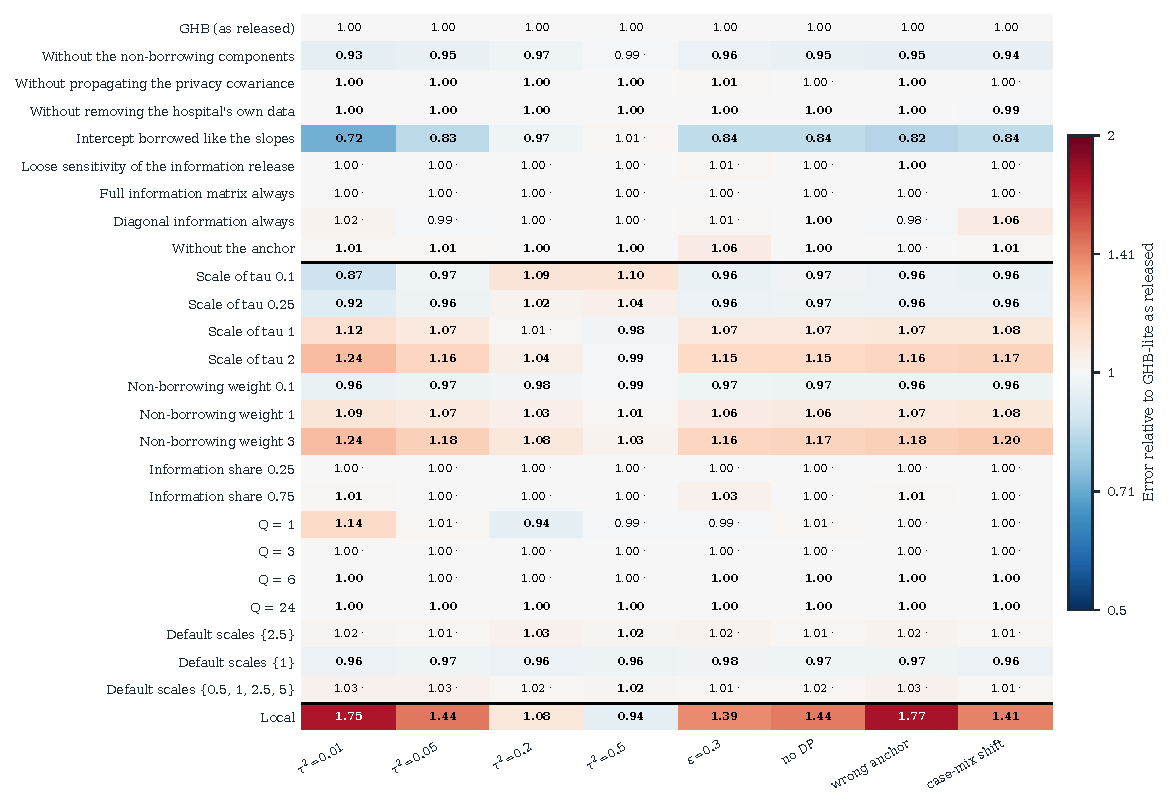
\includegraphics[width=\linewidth]{supplement/figures/sim16_ghb}
\caption{Simulation 16B: ablation (top block) and sensitivity (middle block) of GHB as released (logistic heads, 24 hospitals, \SimSixteenBReps{} replicates per setting). Each cell is the mean excess log-loss of a variant divided by that of GHB on the same data and noise; above 1 (red), the change hurts. Bold: paired difference larger than two standard errors; a trailing dot marks differences within Monte Carlo error. Last row: local estimation, a reference.}
\label{fig:sim-ghb-ablation}
\end{figure}

\subsection{Fairness to groups of patients}\label{sec:sim-fairness}

Every simulation so far asks whether some hospital pays for the others; the last asks whether some group of patients does. In Simulation 18 one feature becomes a protected attribute $S$ whose share varies across hospitals, and its coefficient is each hospital's true disparity, shared, varying, rare or of either sign across hospitals. A variant, \emph{GHB-lite, $S$ local}, keeps the disparity coefficient unborrowed at no privacy cost. FAIR-FATE \cite{salazar2023fairfate}, with its paper's settings, and federated averaging are references: both use a server, FAIR-FATE also a labelled validation set, and neither is private (Figure~\ref{fig:sim-fairness}, Table~\ref{tab:sim18}).

GHB-lite or its variant is the most accurate private method for the minority in every scenario, and the most accurate of all methods whenever hospitals disagree about the disparity. It roughly halves the minority's excess log-loss of local estimation when the disparity is shared (\SimEighteenSharedGHBMin{} against \SimEighteenSharedLocalMin{} $\times10^{-3}$ nats); when disparities vary, single models fit the minority badly (global \SimEighteenVariesGlobalMin, FAIR-FATE \SimEighteenVariesFFEQOMin) while GHB-lite reaches \SimEighteenVariesGHBMin. Because it learns $\tau$ coefficient by coefficient, GHB-lite borrows a disparity hospitals agree on and barely borrows one they disagree on, so keeping it local is a safeguard, not a default. GHB-lite leaves fairness ratios where the true models put them (within 0.02), while FAIR-FATE moves them toward parity, which, when the disparity is real, distorts the minority's predicted risks (\SimEighteenSharedFFEQOMin{} against \SimEighteenSharedGHBMin). Calibrated personalized risk and parity of decisions are different goals, and the choice belongs to the deployment.

\begin{figure}[t]
\centering
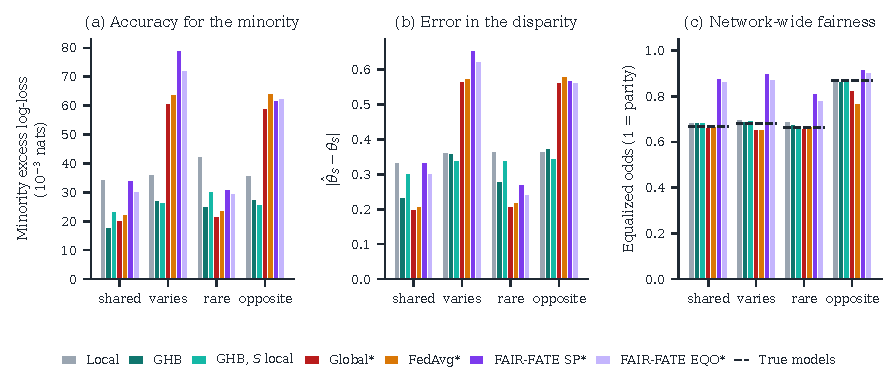
\includegraphics[width=\linewidth]{supplement/figures/sim18_fairness}
\caption{Simulation 18: a protected attribute $S$ ($\epsilon=1$, 24 hospitals, \SimEighteenReps{} replicates per scenario). (a) Mean excess log-loss of the minority group. (b) Mean absolute error of the estimated disparity, the coefficient of $S$. (c) Equalized odds of the network's decisions at threshold 0.5 (1 is parity); dashed: the true models. $\ast$: not private, with a server; FAIR-FATE \cite{salazar2023fairfate} also uses a labelled validation set at the server.}
\label{fig:sim-fairness}
\end{figure}
\begin{table}[t]
\caption{Simulation 18: exact values behind Figure~\ref{fig:sim-fairness} (\SimEighteenReps{} replicates per scenario). Mean excess log-loss over all patients, the minority ($S=1$) and the majority ($10^{-3}$ nats; two standard errors in grey); mean absolute error of the estimated disparity $|\hat\theta_S-\theta_S|$; mean absolute calibration bias in the minority, $|\mathrm{mean}(\hat p-p\mid S=1)|$ (percentage points); the largest ratio of any hospital's excess log-loss to its local one (Worst); and the statistical parity, equal opportunity and equalized odds ratios of the network's decisions at threshold 0.5 (1 is parity). Bold: best of the private methods. $\dagger$: not private, one model trained with a server. FAIR-FATE follows Algorithm~1 of \cite{salazar2023fairfate}: a third of the hospitals per round, 10 local epochs of mini-batch gradient descent (batches of 10, learning rate 0.01), $\lambda_0=0.5$, $\rho=0.05$, $\mathrm{MAX}=0.9$, $\beta_0=0.9$, 100 rounds, and a labelled validation set of a fifth of all patients at the server; federated averaging \cite{mcmahan2017communication} uses the same protocol without the fairness update. All federated models start from the anchor $\mu_0$.}
\label{tab:sim18}
\scriptsize
\setlength{\tabcolsep}{3pt}
\begin{tabular}{@{}lllrrrrrrr@{}}
\toprule
 & \multicolumn{3}{c}{Excess log-loss} & & & & \multicolumn{3}{c}{Fairness of decisions}\\
\cmidrule(lr){2-4}\cmidrule(l){8-10}
Method & All & Minority & Majority & $|\hat\theta_S-\theta_S|$ & \makecell[r]{Calib.\\bias} & Worst & SP & EO & EQO\\
\midrule
\csname @@input\endcsname../Collectively_Big_Locally_Small/supplement/results/tables/t_sim18.tex 
\bottomrule
\end{tabular}
\end{table}
